Given this, it is possible to categorise a theory purely by the composition law it exhibits. 

The recursion can be drawn. Divide a square into four quadrants and
visit them in a fixed order, up the left-hand side, across the top and
down the right-hand side. Divide each quadrant into four again and
visit its sub-squares in the same pattern, rotated or reflected so that
the last sub-square of one quadrant is adjacent to the first sub-square
of the next. After $k$ such steps the path passes once through each of
the $4^k$ cells of a $2^k\times2^k$ grid, moving only between
neighbouring cells. This path is the order-$k$ approximation of the
curve introduced by Hilbert~\cite{hilbert1891stetige}. As $k\to\infty$
it converges to a continuous curve that passes through every point of
the square, the standard example of a space-filling
curve~\cite{haverkort2011inventory}.

Number the cells $1,2,\dots,4^k$ in the order the path visits them, and
take this number as the rank of a symbol. The path finishes each
quadrant before it enters the next, so ranks $1$ to $4^{k-1}$ occupy the
first quadrant, the next $4^{k-1}$ ranks the second, and so on, and the
same holds inside every quadrant at every level. The rank of a cell
therefore specifies a quadrant, then a quadrant within that quadrant,
and so on down to the cell itself. Each quadrant is a register and the
position along the path within it is the symbol, so the subdivision of
Eq.~\eqref{eq:register-subdivision} holds with $n=4^{j}$ at every level
$j$ without reordering any rank. Figure~\ref{fig:register-organisation}(b,c)
shows two organisations of sixteen symbols on the $4\times4$ path, and
Fig.~\ref{fig:refinement-cost-laws}(a) shows the same square described
at successive levels. Because cells that are close along the path are
close in space, these curves are used to order data in spatial
databases and large matrix computations~\cite{haverkort2011inventory}.
For the present argument the curve supplies a concrete organisation in
which each register is a symbol of the level above it. It specifies how
the distinctions nest but not what each level of nesting costs, and
that cost is what $\epsilon$ describes.

The construction does not need the quadrants to fill the square. If
each quadrant is shrunk by a factor $1/s$ with $s>2$ and moved into its
corner, repeating the construction produces a self-similar Cantor dust
of similarity dimension $D=\log4/\log s$. The order in which the cells
are visited is unchanged, and so is every rank and every register.
Figure~\ref{fig:fractional-hilbert} shows this fractional Hilbert order
for dimensions between two, the full square, and one. For $D<2$ the set
consists of disconnected pieces, so no continuous curve can fill it,
and the path drawn in the figure only joins consecutive ranks. The
ordering is all the register hierarchy uses, and it is unaffected.
Space-filling curves on connected self-similar sets have been
constructed systematically~\cite{rao2016spacefilling}. Since
$K_{\mathrm{reg}}(N)$ depends only on the number of distinctions, the
register budget is the same in every panel. The dimension matters only
when distinctions are exchanged for spatial resolution. Resolving a
linear scale $\varepsilon$ requires $N\sim\varepsilon^{-D}$
distinctions, so under homogeneous refinement each $e$-fold improvement
in resolution costs $\kappa D$, a non-integer multiple of $\kappa$
whenever $D$ is not an integer.

\begin{figure*}[t]
  \centering
  \definecolor{fblue}{RGB}{0,114,178}
  \definecolor{forange}{RGB}{230,159,0}
  \definecolor{fink}{RGB}{36,48,57}
  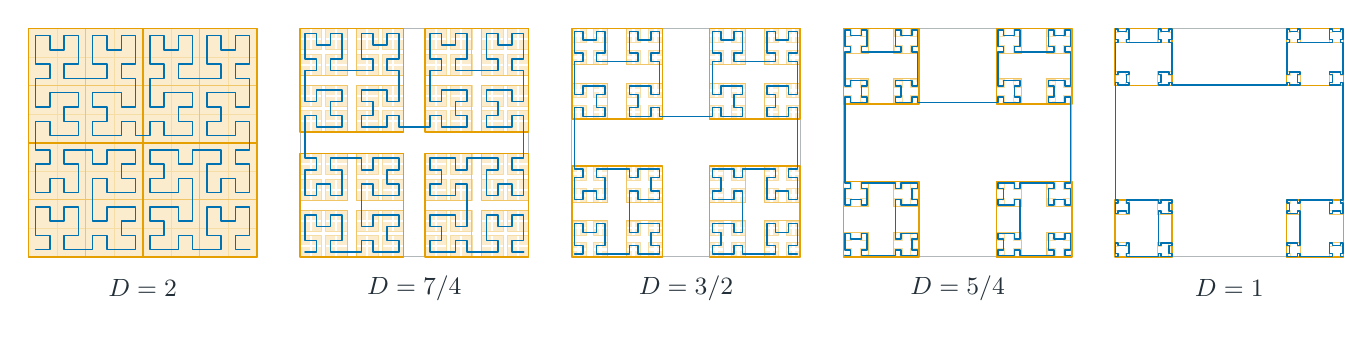
\begin{tikzpicture}[x=1cm,y=1cm,font=\small,line cap=round,line join=round]
  \def\hsq{2.9}
  \def\cpos#1{(\hsq*((1-1/\hs)*(floor((#1)/8)+mod(floor((#1)/4),2)/\hs+mod(floor((#1)/2),2)/(\hs*\hs)+mod((#1),2)/(\hs*\hs*\hs))))}
  \def\cmid#1{(\cpos{#1}+\hsq/(2*\hs*\hs*\hs*\hs))}
  \def\hlist{0/0,0/1,1/1,1/0,2/0,3/0,3/1,2/1,2/2,3/2,3/3,2/3,1/3,1/2,0/2,0/3,0/4,1/4,1/5,0/5,0/6,0/7,1/7,1/6,2/6,2/7,3/7,3/6,3/5,2/5,2/4,3/4,4/4,5/4,5/5,4/5,4/6,4/7,5/7,5/6,6/6,6/7,7/7,7/6,7/5,6/5,6/4,7/4,7/3,7/2,6/2,6/3,5/3,4/3,4/2,5/2,5/1,4/1,4/0,5/0,6/0,6/1,7/1,7/0}
  \foreach \Dval/\Dlab [count=\p from 0] in {2/{2},1.75/{7/4},1.5/{3/2},1.25/{5/4},1/{1}} {
   \pgfmathsetmacro\hs{pow(4,1/\Dval)}
   \begin{scope}[shift={(\p*3.45,0)}]
    \draw[fink!35,line width=0.4pt] (0,0) rectangle (\hsq,\hsq);
    \foreach \i in {0,...,15} \foreach \j in {0,...,15} {
      \pgfmathsetmacro\xc{\cpos{\i}}
      \pgfmathsetmacro\yc{\cpos{\j}}
      \fill[forange!20] (\xc,\yc) rectangle ++({\hsq/(\hs*\hs*\hs*\hs)},{\hsq/(\hs*\hs*\hs*\hs)});
    }
    \foreach \i in {0,...,7} \foreach \j in {0,...,7} {
      \pgfmathsetmacro\xb{\hsq*(1-1/\hs)*(floor(\i/4)+mod(floor(\i/2),2)/\hs+mod(\i,2)/(\hs*\hs))}
      \pgfmathsetmacro\yb{\hsq*(1-1/\hs)*(floor(\j/4)+mod(floor(\j/2),2)/\hs+mod(\j,2)/(\hs*\hs))}
      \draw[forange!35,line width=0.25pt] (\xb,\yb) rectangle ++({\hsq/(\hs*\hs*\hs)},{\hsq/(\hs*\hs*\hs)});
    }
    \foreach \i in {0,...,3} \foreach \j in {0,...,3} {
      \pgfmathsetmacro\xb{\hsq*(1-1/\hs)*(floor(\i/2)+mod(\i,2)/\hs)}
      \pgfmathsetmacro\yb{\hsq*(1-1/\hs)*(floor(\j/2)+mod(\j,2)/\hs)}
      \draw[forange!60,line width=0.35pt] (\xb,\yb) rectangle ++({\hsq/(\hs*\hs)},{\hsq/(\hs*\hs)});
    }
    \foreach \i in {0,1} \foreach \j in {0,1} {
      \pgfmathsetmacro\xa{\hsq*(1-1/\hs)*\i}
      \pgfmathsetmacro\ya{\hsq*(1-1/\hs)*\j}
      \draw[forange,line width=0.6pt] (\xa,\ya) rectangle ++({\hsq/\hs},{\hsq/\hs});
    }
    \draw[fblue,line width=0.55pt] ({\cmid{0}},{\cmid{0}})
      \foreach \i/\j in \hlist { -- ({\cmid{\j}},{\cmid{\i}}) }
      \foreach \i/\j in \hlist { -- ({\cmid{\i}},{\cmid{\j+8}}) }
      \foreach \i/\j in \hlist { -- ({\cmid{\i+8}},{\cmid{\j+8}}) }
      \foreach \i/\j in \hlist { -- ({\cmid{15-\j}},{\cmid{7-\i}}) };
    \node[text=fink] at (\hsq/2,-0.4) {$D=\Dlab$};
   \end{scope}
  }
  \end{tikzpicture}
  \caption{\textbf{The Hilbert order at non-integer dimension.} The
    order-four Hilbert sequence of $N=4^4$ ranks, with its nested
    registers, placed on the self-similar set generated by four corner
    maps of ratio $1/s$, where $s=4^{1/D}$. Orange outlines mark the
    registers at depths one to three, and shaded cells the individual
    symbols. The panel $D=2$ is Hilbert's square. For $D<2$ the set is
    totally disconnected and the blue path is a guide joining
    consecutive ranks rather than part of the set. The ranks, the
    nesting and the register budget are identical in every panel.}
  \label{fig:fractional-hilbert}
\end{figure*}